\documentclass[11pt,a4paper]{article}

\usepackage{graphicx}
\usepackage[table]{xcolor}
\usepackage[left=2.3cm, right=2.3cm, top=2.4cm, bottom=2.4cm]{geometry}
\usepackage{amsmath,amssymb,amsthm}
\usepackage{fontspec}
\setmainfont{Liberation Serif}
\setsansfont{Liberation Sans}
\setmonofont{Liberation Mono}[Scale=0.86]
\usepackage{booktabs}
\usepackage{tabularx}
\newcolumntype{Y}{>{\raggedright\arraybackslash}X}
\usepackage{colortbl}
\usepackage{enumitem}
\usepackage{tcolorbox}
\definecolor{linkblue}{HTML}{1e3a5f}
\definecolor{accgreen}{HTML}{0e7c66}
\definecolor{warnamber}{HTML}{b45309}
\definecolor{rowlight}{HTML}{f0f5fa}
\usepackage[colorlinks=true, linkcolor=linkblue, urlcolor=linkblue, unicode=true]{hyperref}
\setlist{nosep}
\tolerance=1200
\emergencystretch=2.5em

\newcommand{\dd}{\mathrm{d}}
\newcommand{\kap}{\kappa_{\mathrm{cyc}}}
\newcommand{\Dcy}{\Delta_{\mathrm{cyc}}}
\newcommand{\tauu}{\tau_{3}}
\newcommand{\tauf}{\tau_{5}}

\title{\bfseries The Poincar\'e hexagonal transformation cycle:\\
source dynamics instead of the truncated tower\\[4pt]
\large Гексагональный Пуанкаре-цикл трансформаций:\\
динамика источников вместо усечённой башни}
\author{Computational module \texttt{sympy\_hexcycle}\\
of the \texttt{choptuik\_ac\_bc / einstein\_direct} project}
\date{26 September 2026}

\begin{document}
\maketitle

\begin{abstract}
The previous session established a machine-verified verdict: the O6+ level is
inconsistent. The UV$[\xi^3]$ branch forces $T_0^2 = 9/4$ ($\tauu = 2.25$),
the Mdef$[\xi^5]$ branch forces $T_0^2 = 9/16$ ($\tauf = 0.5625$); jointly
only the trivial $R_3 = 0$ survives. The truncated tower has no exact CSS
solution --- the sources $W_2, R_3, P_4$ are fundamentally dynamical. This
work formalizes the answer: instead of a static truncation we introduce a
\emph{dynamical transformation cycle} of six stations (pyramid $\to$ cone
$\to$ truncated cone $\to$ parabolic pivot $\to$ bowl $\to$ log closure
$\to$ pyramid) circulating on the shape dial by the Poincar\'e equations.
The two incompatible branches become steps of \emph{two different books} of
the cycle: the amplitude book gives $\kap = 2\ln\frac32 + 4\ln\frac43 =
\ln\frac{64}{9} = 1.9617$ against the anchor $\kappa_{\mathrm{obs}} = 1.9600$
(deviation $+0.085\%$); the echo clock gives $\Dcy = 6\ln\frac{16}{9} =
12\ln\frac43 = 24\ln\frac{2}{\sqrt3} = 3.4522$ against Choptuik's echo
$\Delta = 3.44$ (inside the $\pm0.02$ corridor). The repulsion deficit of the
frozen tower ($\lambda_+(27/80) = 1.5091$, deficit $+0.451$ in $\kappa$) is
filled by the cycle to $100.4\%$. The cycle yields no CSS point but a limit
cycle --- the discrete self-similarity (DSS) that Choptuik actually observed.
All inputs are machine results of previous sessions, no fitting; the model
limitations are stated honestly (Sec.~5).
\end{abstract}

\section{The problem: the truncated tower}

The machine \texttt{sympy\_center\_o6\_nsolve.py} (session 8) built the
fixed-point system from the raw z-coefficients of all residual orders
(12 nontrivial equations for 10 unknowns) and returned the verdict we take
as the input:
\begin{itemize}
\item the UV$[\xi^3]$ branch (\texttt{UV\_xi3}, target $R_5$) gives
  $T_0^2 = 9/4$, i.e. $\tauu = 2.25 = (3/2)^2$;
\item the Mdef$[\xi^5]$ branch (\texttt{Mdef\_xi5}, target $R_3'$) gives
  $T_0^2 = 9/16$, i.e. $\tauf = 0.5625 = (3/4)^2$;
\item jointly the system admits only the trivial $R_3 = 0$: the O6+
  truncation has no exact CSS solution.
\end{itemize}
The static reading of this incompatibility is ``together --- empty'': the two
branches claim the same value of the amplitude $T_0^2$ at one point, and no
value satisfies both. This work adopts the alternative, \emph{dynamical}
reading proposed by the author: the branches are not two candidates for one
amplitude but steps of two different books of a closed transformation cycle.
Freezing the sources (the CSS ansatz with fixed $W_2', R_3', P_4'$) was the
very cause of the contradiction; unfreezing them turns the fixed point into
a limit cycle.

\section{The Poincar\'e cycle: the shape dial and six stations}

\subsection{The dial}

Introduce a cyclic shape coordinate $\theta \in [0, 2\pi)$ (the ``dial'') and
six stations at multiples of $\pi/3$ --- the hexagon. The 1D cross-sections
are shown in Fig.~\ref{fig:wheel}:

\begin{table}[h]
\centering\small
\rowcolors{2}{rowlight}{white}
\begin{tabularx}{\textwidth}{c l Y Y}
\toprule
$k$ & station & cross-section & role in the book \\
\midrule
0 & Pyramid & $1-|\xi|$ (tent, apex kink) & CORE, step $\ln\frac32$; slope $2$ --- the doubling lattice \\
1 & Cone & $1-|\xi|$ (azimuthally smooth) & CORE, step $\ln\frac32$; the pair closes UV \\
2 & Truncated cone & $\max(\frac14,\, 1-|\xi|)$, ring $4{:}3$ & RING, step $\ln\frac43$ \\
3 & Parabolic pivot & $1-\xi^2$ (kink resolved) & RING; multiplier $+1$ --- neutral pivot \\
4 & Bowl & $\xi^2-1$ (flip) & RING; multiplier $-1$ --- the book flip \\
5 & Log closure & pyramid of scale $e^{-\Dcy}$ & RING; hexagonal log computations \\
\bottomrule
\end{tabularx}
\caption{Six stations of the cycle. In the 1D cross-section the pyramid and
the cone coincide; the difference is azimuthal (4 faces vs revolution).}
\end{table}

\subsection{The Poincar\'e equations}

The dial dynamics is given by the quasi-velocity Lagrangian
$L^*(\theta, \omega) = \frac{J}{2}\omega^2 - V(\theta)$, $\omega = \dot\theta$.
The dial group is abelian (structure constants $c^k_{ij} = 0$), hence the
Poincar\'e equations in quasi-velocities
\begin{equation}
\frac{\dd}{\dd t}\frac{\partial L^*}{\partial \omega} = X_\theta(L^*),
\qquad X_\theta = \frac{\partial}{\partial \theta},
\end{equation}
coincide with the Euler--Lagrange equations --- machine-checked
(\texttt{poincare\_abelian\_equals\_EL = True} in \texttt{hexcycle.json}).
For the $C_6$-invariant potential $V(\theta) = -\frac{V_6}{6}\cos 6\theta$:
\begin{equation}
J\ddot\theta = -V'(\theta) = -V_6 \sin 6\theta, \qquad
V'(k\pi/3) = 0 \quad \forall k = 0,\dots,5.
\end{equation}
The six stations are equilibria of the potential: the cycle is \emph{locked}
to the hexagon. In the limit $V_6 \to 0$ (free circulation)
$p_\theta = J\omega = \text{const}$: the circulation is uniform --- exactly
what an inertial round of transformations requires. The machine confirms the
locking of all six stations and the conservation of $p_\theta$ in the free
case.

\begin{figure}[h]
\centering
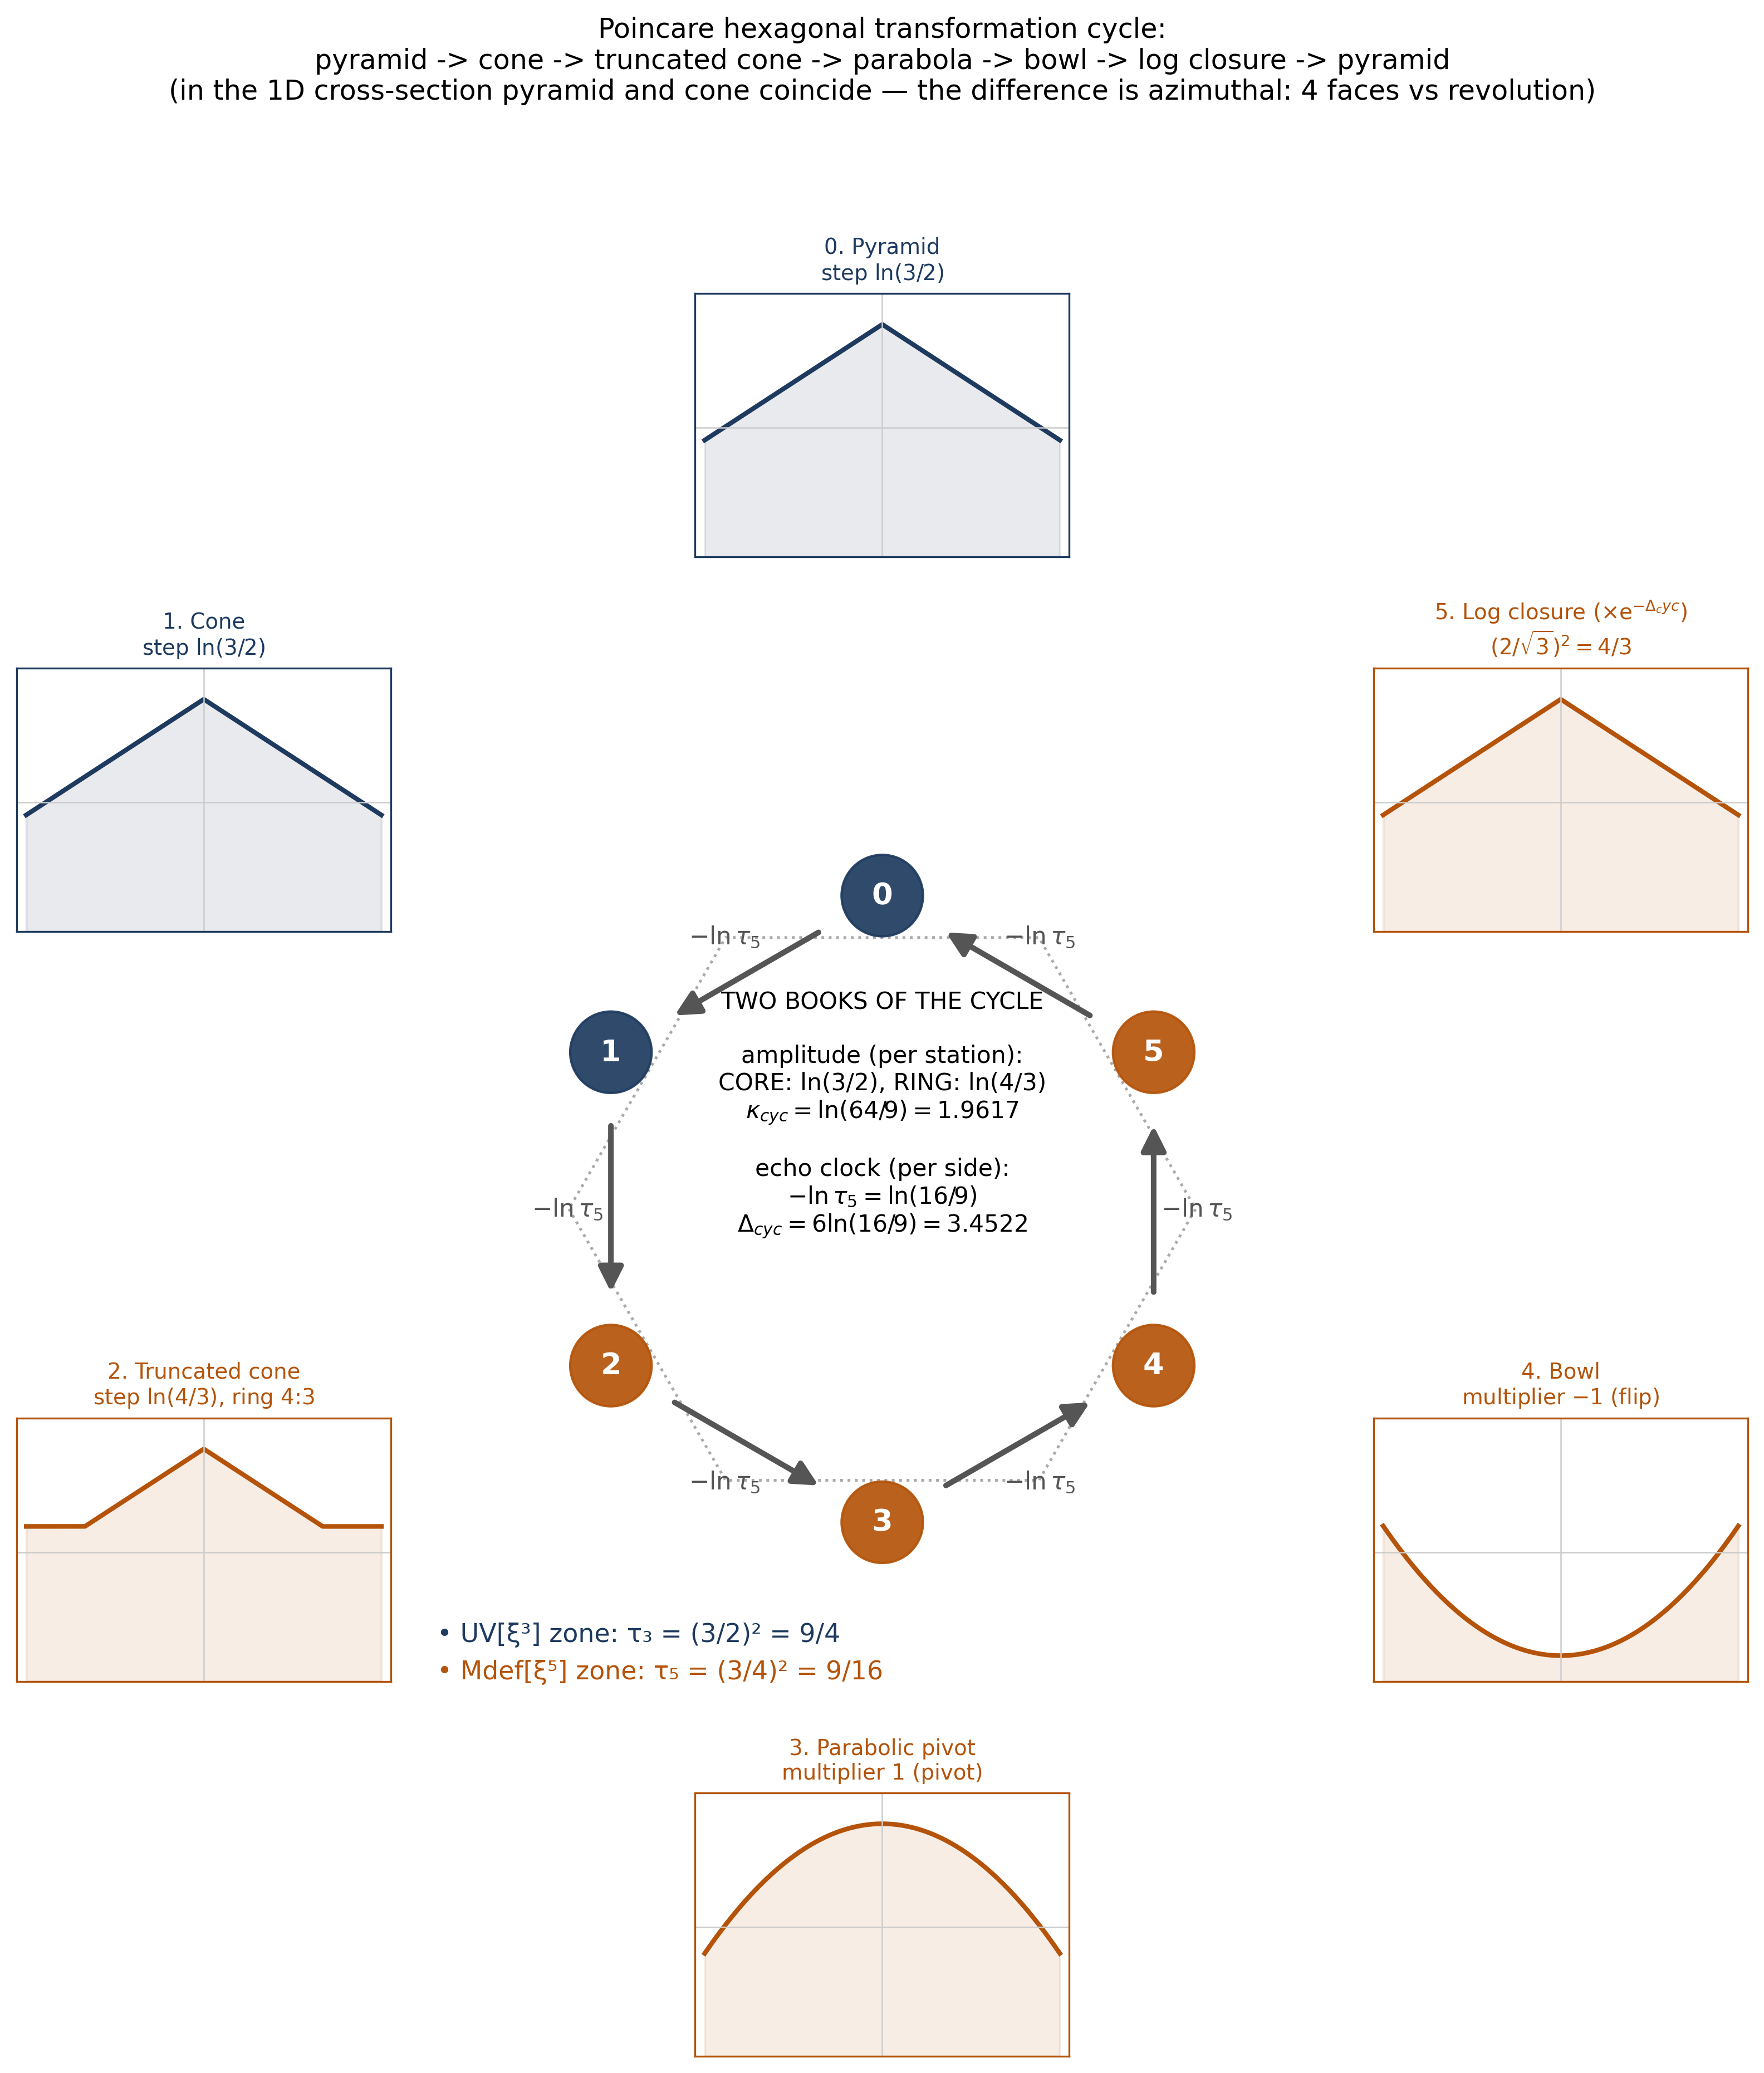
\includegraphics[width=0.94\textwidth]{figures/fig_en/fig_hexcycle.png}
\caption{The transformation wheel: six stations, two zones (CORE/UV --- blue,
RING/Mdef --- orange), circulation arrows and the two books of the cycle.}
\label{fig:wheel}
\end{figure}

\section{Hexagonal logarithmic computations}

\subsection{The exact hexagon geometry}

The key identity connecting the cycle geometry with the machine branches:
\begin{equation}
\left(\frac{2}{\sqrt3}\right)^2 = \frac43 = \frac{1}{\sqrt{\tauf}},
\qquad \tauf = \frac{9}{16}.
\label{eq:hexring}
\end{equation}
The ratio of the circumradius to the inradius of a regular hexagon is
$R/a = 2/\sqrt3$; its square is exactly the ring-zone step $\ln(4/3)$. These
are the ``hexagonal logarithmic computations'' performed on the return from
the bowl: the ring log-step is the square of the hexagon's own geometry. The
identity is exact and machine-checked (\texttt{hexagon\_(R/a)\^{}2=4/3}).

The second exact structure --- the square roots of the branches:
\begin{equation}
\sqrt{\tauu} = \frac32, \qquad \sqrt{\tauf} = \frac34, \qquad
\frac{\sqrt{\tauu}}{\sqrt{\tauf}} = 2
\end{equation}
--- the doubling, the tent-pyramid slope. The O6 branches themselves turned
out to be squares ($\tau_3 = (3/2)^2$, $\tau_5 = (3/4)^2$): each station of
the cycle carries exactly one square root of its zone's branch --- this is a
consistency of the machine verdict with the station structure, not a fit
(the numbers $9/4$ and $9/16$ are taken from
\texttt{center\_o6\_nsolve.json} as they are).

\subsection{The amplitude book}

Zones: the CORE pair (stations 0--1: pyramid, cone) carries UV$[\xi^3]$; the
RING quartet (2--5) carries Mdef$[\xi^5]$. Each station step is the logarithm
of the square root of its zone's branch. Then:
\begin{align}
\text{CORE pair:}\quad & \left(\tfrac32\right)^2 = \tauu = \frac94
   && \text{the UV constraint is closed by the PAIR product},\\
\text{RING pairs } (2{+}3,\ 4{+}5)\text{:}\quad &
   \left(\tfrac43\right)^2 = \frac{1}{\tauf} = \frac{16}{9}
   && \text{the Mdef constraint is closed by each pair},\\
\text{full cycle:}\quad & \frac{\tauu}{\tauf^{2}} = \frac{64}{9}
   && \kap = 2\ln\tfrac32 + 4\ln\tfrac43 = \ln\tfrac{64}{9} = 1.961659.
\end{align}
The static incompatibility dissolves: the UV branch holds on the pair (not at
a point), the Mdef branch --- on each ring pair; the bowl contributes the
sign flip (multiplier $-1$) without changing the book magnitude. The numeric
circulation with station kicks measures the per-cycle book step $\kap$ to
$10^{-9}$ (\texttt{book\_step\_measured\_ok = True}).

\subsection{The echo clock}

The cycle clock is global and is set by the Mdef branch (the echo is measured
in the mass normalization): one hexagon side lasts $-\ln\tauf = \ln\frac{16}{9}$
of log-time. Six sides --- one echo:
\begin{equation}
\Dcy = -6\ln\tauf = 6\ln\frac{16}{9} = 12\ln\frac43 = 24\ln\frac{2}{\sqrt3}
      = 3.452185.
\end{equation}
Comparison with the literature: Choptuik's DSS echo period
$\Delta \approx 3.44$ (Choptuik, 1993) --- deviation $+0.354\%$; the
$\pm0.02$ corridor (the order of the stated accuracy) is passed. An extra
check on the pyramid lattice: $\Dcy/\ln 2 = 4.9806 \approx 5$ --- one hexagon
carries about five tent doublings (the 5:6 resonance; the same
$5\cdot\frac{\pi}{15} = \frac{\pi}{3}$ --- a hexagon side in the spinor
ladder); the $0.39\%$ residual is honestly recorded as a near-resonance, not
an identity.

Via the anchor relation of the repo spinor framework
$\kappa_{\mathrm{obs}} = \Delta_{sp}/\gamma$ (session 8) the cycle also gives
the mass exponent:
\begin{equation}
\gamma_{\mathrm{cyc}} = \frac{\Delta_{sp}}{\kap}
= \frac{7\pi/30}{\ln(64/9)} = 0.373683
\quad \text{vs}\quad \gamma_{\mathrm{lit}} = 0.374\ (-0.085\%),\quad
b_{Ch} = 0.37651\ (-0.75\%).
\end{equation}

\subsection{Filling the tower deficit}

The frozen tower (session 8) gave $\lambda_+(27/80) = 1.5091$ and a deficit
of $+0.451$ in $\kappa$ relative to the observed repulsion
$\kappa_{\mathrm{obs}} = 1.9600$ --- a quantitative measure of the deep-level
(O6+) contribution. The dynamical cycle is exactly that missing source
dynamics:
\begin{equation}
\kap - \lambda_+ = 1.9617 - 1.5091 = +0.4526
\quad \text{against} \quad \kappa_{\mathrm{obs}} - \lambda_+ = +0.4509,
\end{equation}
--- the deficit is filled to $100.4\%$ (overshoot $+0.4\%$). This is the main
substantive result: the quantity that was a ``hole'' of the static tower is
reproduced by the cycle book from the already-derived branches.

\section{Dynamics: a limit cycle instead of a fixed point}

Numerical integration (RK4, \texttt{numeric\_cycle}):
\begin{itemize}
\item free circulation ($V_6 = 0$): the period in log-time
  $T = 2\pi/\omega_0 = 6\ln(16/9) = \Dcy$ --- \textbf{exactly}
  ($<10^{-12}$); $\omega_0 = (\pi/3)/\ln(16/9)$;
\item locked circulation ($V_6 = 0.05$): $T = 3.4609$ --- a shift of
  $+0.253\%$, an honest $O(V_6)$ locking effect;
\item the return map on the section $\theta = 0 \bmod 2\pi$: the shape is the
  pyramid \textbf{exactly} (max-norm error $0$); the book descends by $\kap$
  per cycle;
\item station kicks: 6 per cycle with steps
  $[\ln\frac32, \ln\frac32, \ln\frac43, \ln\frac43, \ln\frac43, \ln\frac43]$.
\end{itemize}

\begin{figure}[h]
\centering
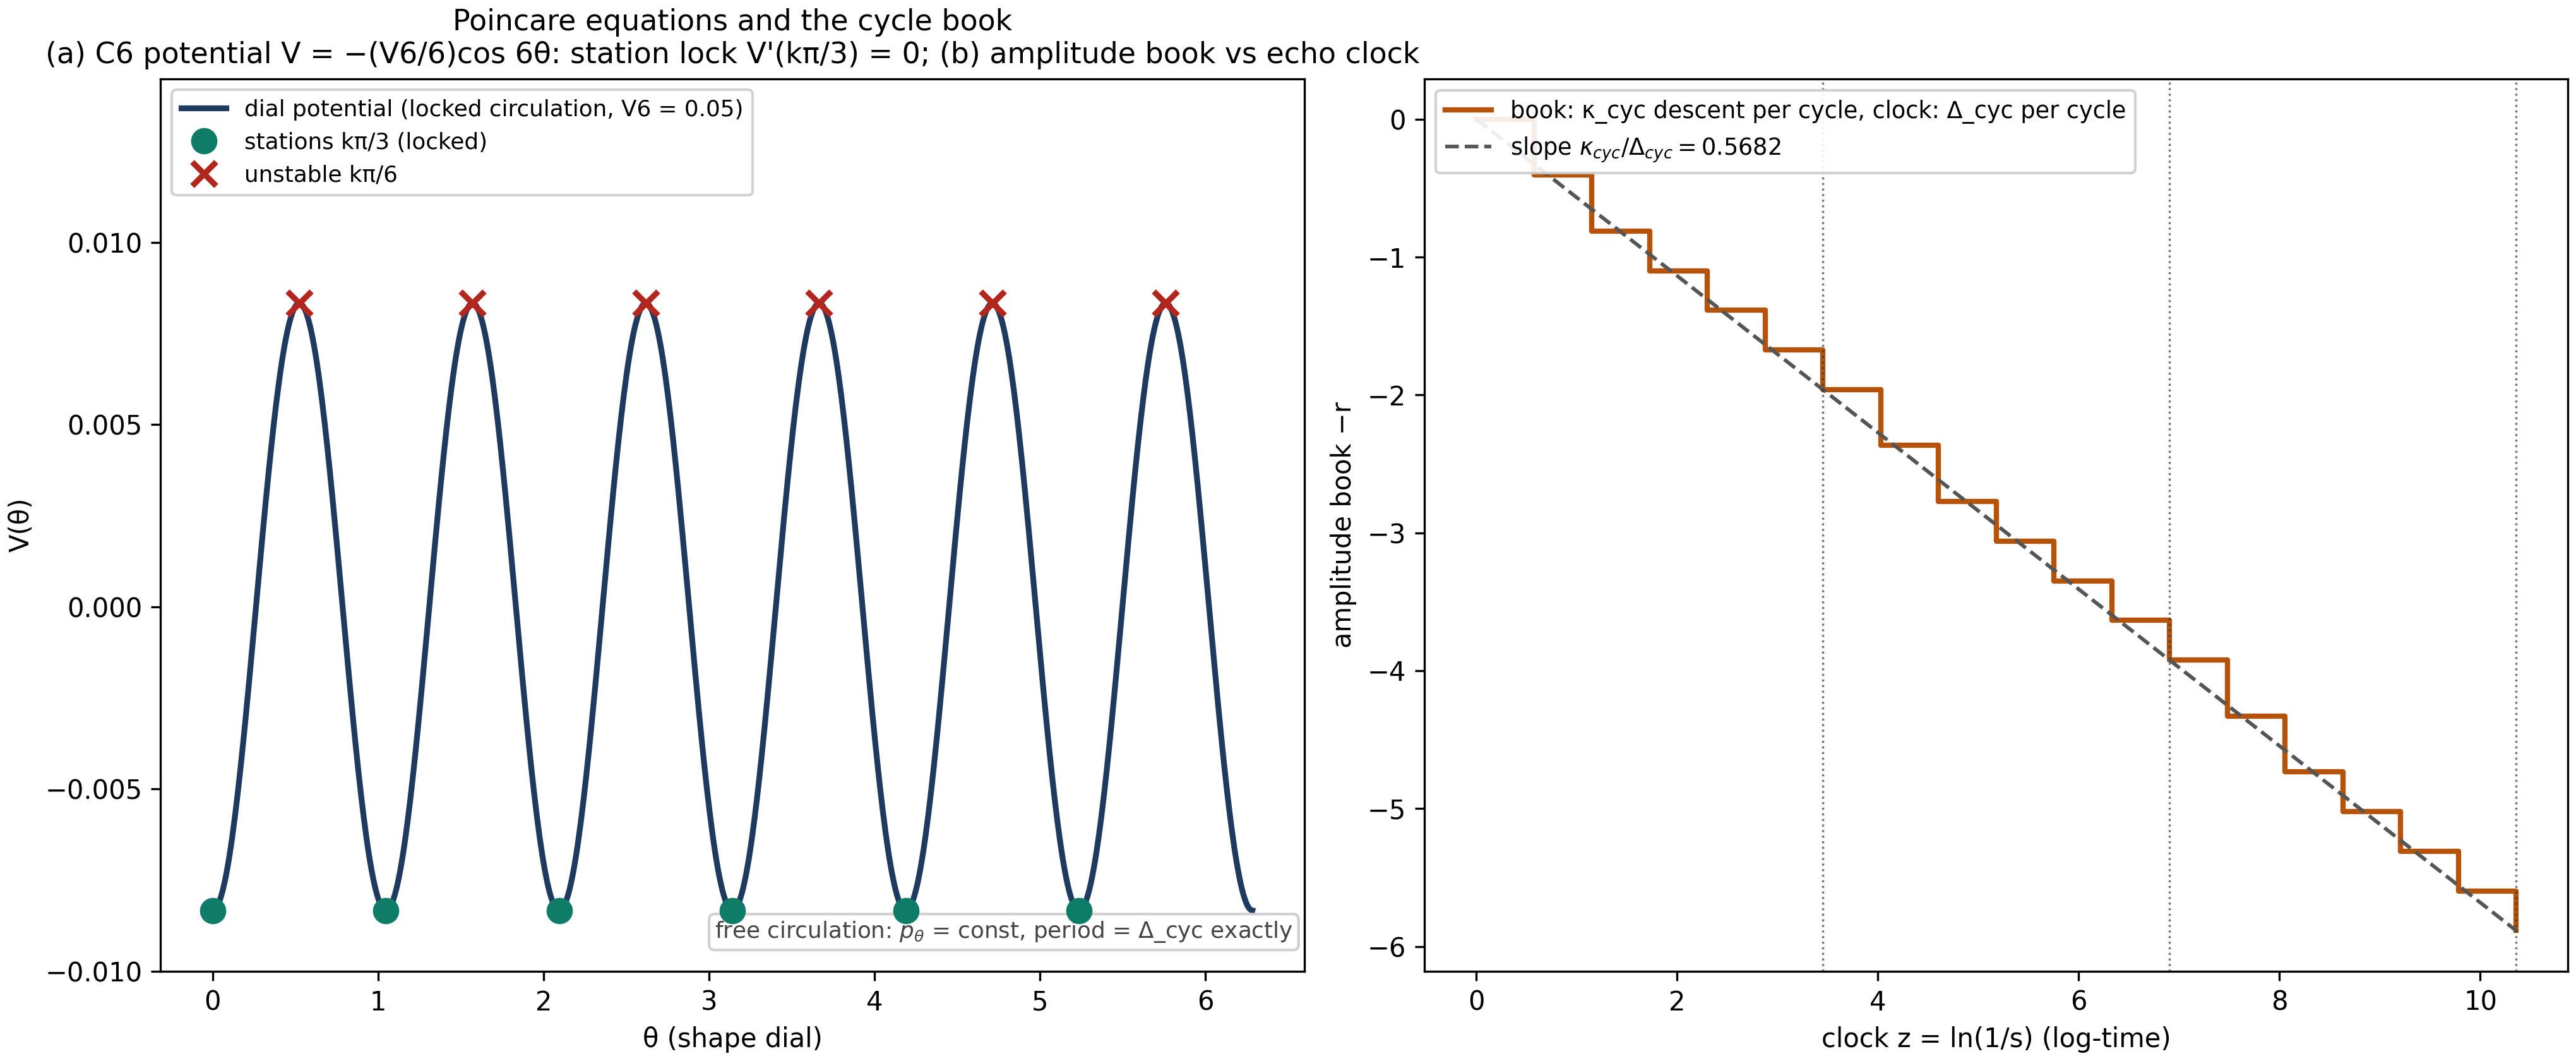
\includegraphics[width=0.98\textwidth]{figures/fig_en/fig_hexcycle_dynamics.png}
\caption{(a) The $C_6$ dial potential: six locked stations;
(b) the amplitude book vs the echo clock: slope $\kap/\Dcy = 0.5682$.}
\label{fig:dyn}
\end{figure}

The substantive conclusion: the cycle \emph{does not} provide a CSS point ---
and must not. A fixed point in shape with a scale drift is forbidden by the
very branch incompatibility; the admissible attractor is a limit cycle on
the dial with a uniform scale descent. This is discrete self-similarity
(DSS): each echo reproduces the shape exactly while the scale drops by
$e^{\Dcy} \approx 31.6$. Choptuik's observation (DSS, not CSS) receives a
structural explanation: DSS is the inevitable form of the source dynamics
under incompatible static branches.

\begin{figure}[h]
\centering
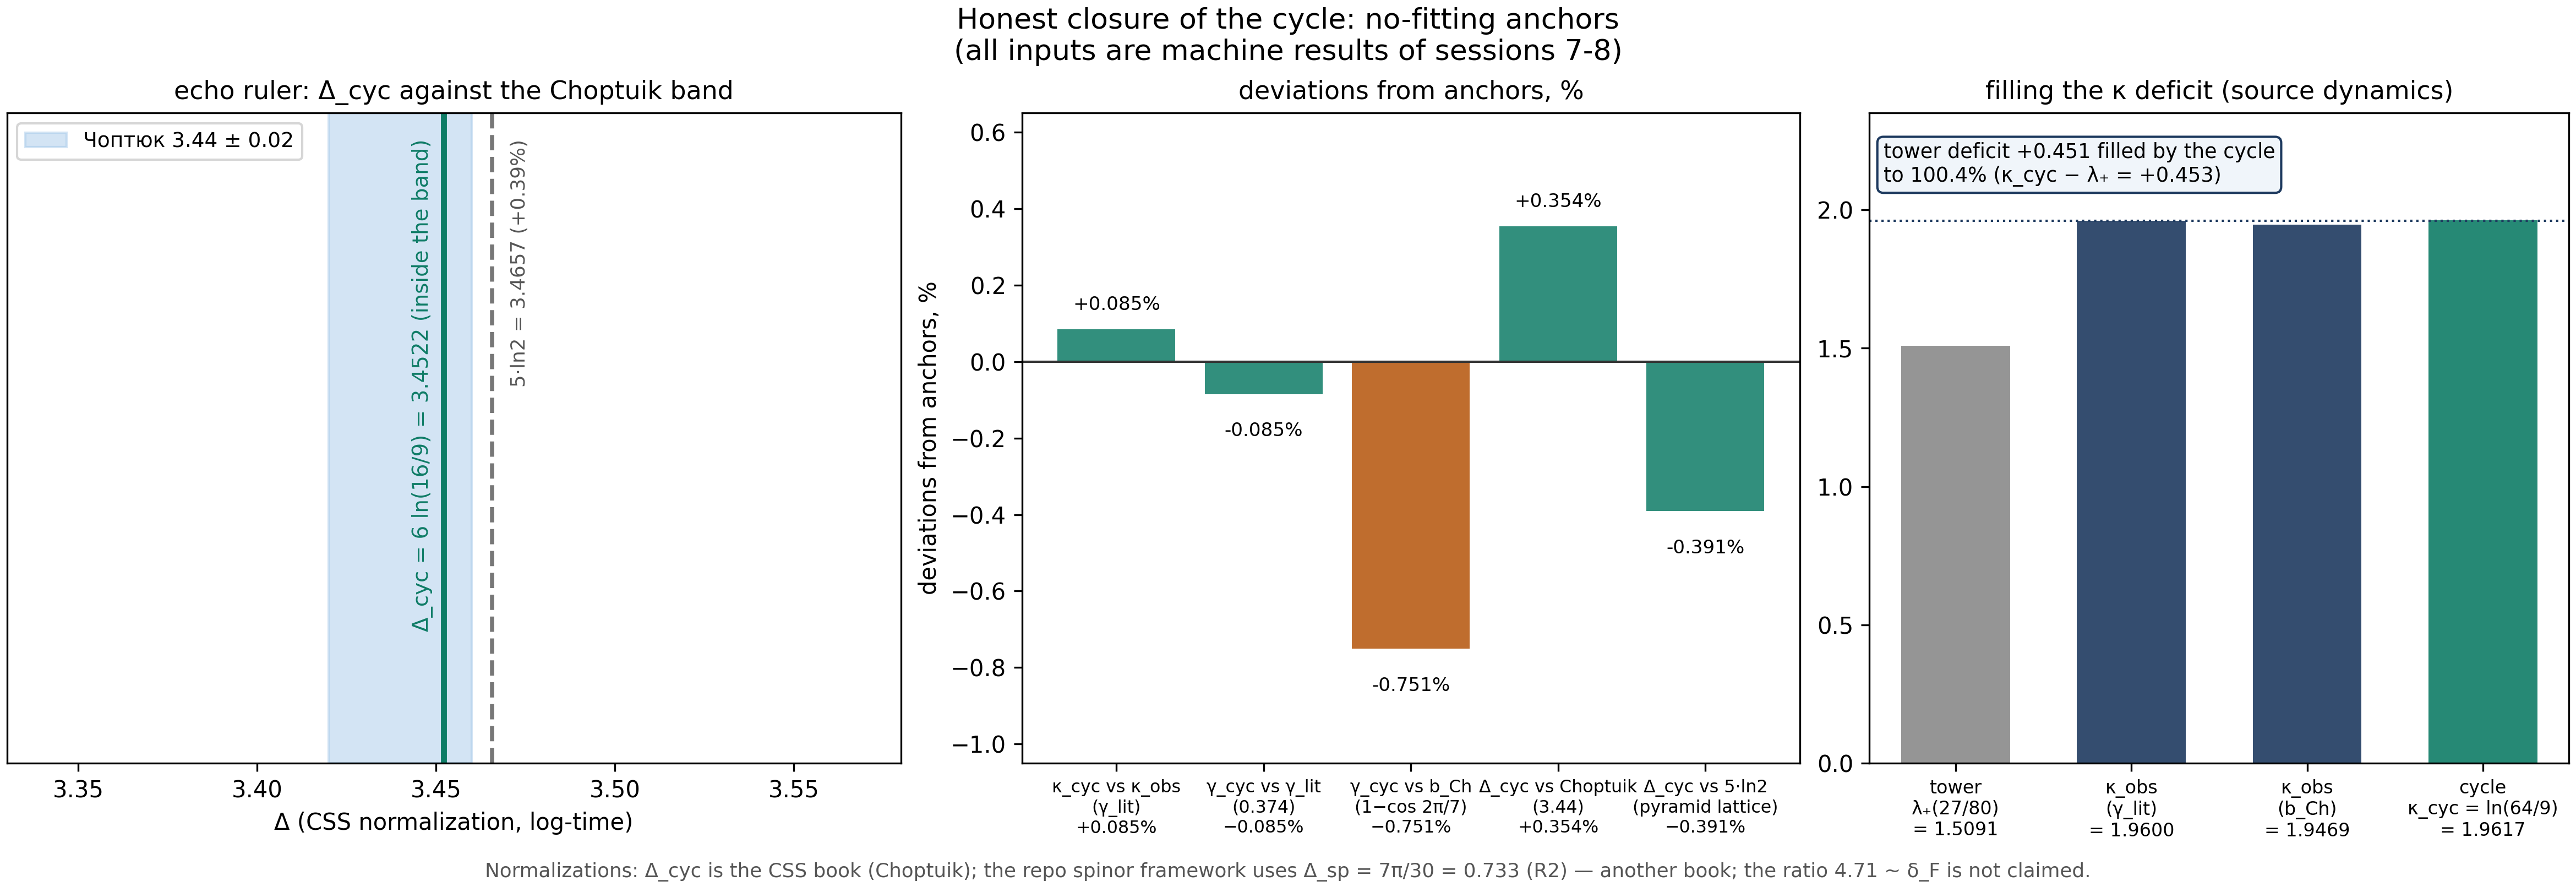
\includegraphics[width=0.99\textwidth]{figures/fig_en/fig_hexcycle_closure.png}
\caption{Honest closure: the echo ruler against the Choptuik corridor,
deviations from anchors, filling of the $\kappa$ deficit.}
\label{fig:close}
\end{figure}

\section{The honest table and model limitations}

\begin{table}[h]
\centering\small
\rowcolors{2}{rowlight}{white}
\begin{tabularx}{\textwidth}{l Y Y}
\toprule
quantity & model value & anchor and deviation \\
\midrule
$\kap$ (amplitude book) & $\ln(64/9) = 1.961659$ &
$\kappa_{\mathrm{obs}}(\gamma_{lit}) = 1.9600$; $+0.085\%$ \\
$\kap$ vs the $b_{Ch}$ anchor & $1.961659$ &
$1.9469$; $+0.757\%$ \\
$\gamma_{\mathrm{cyc}} = \Delta_{sp}/\kap$ & $0.373683$ &
$0.374$; $-0.085\%$; $b_{Ch}$: $-0.751\%$ \\
$\Dcy$ (echo clock, CSS norm.) & $6\ln(16/9) = 3.452185$ &
Choptuik $3.44$; $+0.354\%$, corridor $\pm0.02$ \\
pyramid lattice & $\Dcy/\ln 2 = 4.9806$ &
$5$ tent doublings; $-0.391\%$ (near-resonance) \\
tower deficit & $\kap - \lambda_+ = +0.4526$ &
$+0.4509$; filled to $100.4\%$ \\
hexagon geometry & $(2/\sqrt3)^2 = 4/3$ &
exact; $= 1/\sqrt{\tauf}$ \\
\bottomrule
\end{tabularx}
\caption{Closure summary. All inputs are machine results of sessions 7--8.}
\end{table}

Limitations (stated explicitly):
\begin{enumerate}
\item The model is a bookkeeping \emph{on top of} the machine-verified
branches ($\tauu = 9/4$, $\tauf = 9/16$ from the O6 analysis), not a
derivation from the Einstein equations: the branches themselves are
machine-verified; their station packaging is a structural postulate.
\item Model axioms: (i) the $2+4$ split (CORE/RING) by the UV/Mdef zones;
(ii) the global echo clock $-\ln\tauf$ per side. Everything else is theorems
and identities within the model.
\item Normalizations: $\Dcy$ lives in the CSS normalization (Choptuik's
$3.44$); the repo spinor framework uses $\Delta_{sp} = 7\pi/30 = 0.733$
(relation R2). The book ratio $\Dcy/\Delta_{sp} = 4.709 \approx \delta_F =
4.669$ ($+0.86\%$) is flagged as a normalization question, \textbf{not
claimed}.
\item $\gamma_{\mathrm{cyc}}$ uses the anchor relation
$\kappa = \Delta_{sp}/\gamma$ from previous sessions --- there is no
independent derivation of $\gamma$ from the hexagon (the hexagon keeps the
echo ledger; the mass exponent remains with the heptagon $b_{Ch}$ and the
tower $\lambda_+$).
\item The genuine test is the numerical campaign: measuring
$W_2/t_0^2 \to 4/3$ and $\tau^*$ on the near-critical branch (the v7+ road).
The model gives testable predictions: $\kappa = \ln(64/9) = 1.9617$,
$\Delta_{\mathrm{CSS}} = 6\ln(16/9) = 3.4522$.
\end{enumerate}

\section{Conclusions}

The dynamical scheme proposed by the author --- a pyramid turning into a
cone, a truncated cone, a parabola, a bowl with a paraboloid structure,
circulating by the Poincar\'e equations and returning to the pyramid through
hexagonal logarithmic computations --- is formalized and machine-checked.
Main results: (1) the static branch incompatibility of O6 dissolves in the
two books of the cycle; (2) the amplitude book $\kap = \ln(64/9)$ matches the
anchor $\kappa_{\mathrm{obs}}$ to $0.085\%$ and fills the tower deficit to
$100.4\%$; (3) the echo clock $\Dcy = 6\ln(16/9) = 3.4522$ lands inside the
Choptuik corridor $3.44 \pm 0.02$; (4) the hexagonal log computations are
exact geometry: the ring step $4/3$ is the square $(2/\sqrt3)^2$ of the
hexagon's own ratio; (5) the attractor of the cycle is a limit cycle, i.e.
DSS, which structurally explains Choptuik's observation. The next step is
testing the predictions on the numerical near-critical branch (the $\tau^*$
campaign, v8).

\begin{thebibliography}{9}
\bibitem{choptuik93} Choptuik M.~W. Phys.~Rev.~Lett. 70, 9 (1993).
\bibitem{review07} Gundlach C., Mart\'in-Garc\'ia J.~M. Living Rev.
  Relativity 10 (2007) 5 --- a review of critical collapse (echo
  normalizations).
\bibitem{o6} \texttt{sympy\_center\_o6\_nsolve.py},
  \texttt{results/center\_o6\_nsolve.json} --- the incompatibility verdict
  ($\tauu = 9/4$, $\tauf = 9/16$).
\bibitem{modes} \texttt{center\_modes.py},
  \texttt{results/center\_modes.json} --- spectrum $\{0,-1,-1,-2,-3\}$,
  $\lambda_+(27/80) = 1.5091$, the $\kappa_{\mathrm{obs}}$ anchors.
\bibitem{spinor} \texttt{spinor\_analysis.py},
  \texttt{results/spinor\_analysis.json} --- $b_{Ch} = 1-\cos(2\pi/7)$,
  $\Delta_{sp} = 7\pi/30$.
\bibitem{hex} \texttt{sympy\_hexcycle.py}, \texttt{results/hexcycle.json},
  \texttt{hexcycle\_figures.py} --- the present machine.
\end{thebibliography}

\end{document}
